% THIS IS SIGPROC-SP.TEX - VERSION 3.1
% WORKS WITH V3.2SP OF ACM_PROC_ARTICLE-SP.CLS
% APRIL 2009
%
% It is an example file showing how to use the 'acm_proc_article-sp.cls' V3.2SP
% LaTeX2e document class file for Conference Proceedings submissions.
% ----------------------------------------------------------------------------------------------------------------
% This .tex file (and associated .cls V3.2SP) *DOES NOT* produce:
%       1) The Permission Statement
%       2) The Conference (location) Info information
%       3) The Copyright Line with ACM data
%       4) Page numbering
% ---------------------------------------------------------------------------------------------------------------
% It is an example which *does* use the .bib file (from which the .bbl file
% is produced).
% REMEMBER HOWEVER: After having produced the .bbl file,
% and prior to final submission,
% you need to 'insert'  your .bbl file into your source .tex file so as to provide
% ONE 'self-contained' source file.
%
% Questions regarding SIGS should be sent to
% Adrienne Griscti ---> griscti@acm.org
%
% Questions/suggestions regarding the guidelines, .tex and .cls files, etc. to
% Gerald Murray ---> murray@hq.acm.org
%
% For tracking purposes - this is V3.1SP - APRIL 2009

\documentclass{edm_article}



\begin{document}

\title{The Effect of an Intelligent Tutor on Performance on Specific Posttest Problems\titlenote{(Does NOT produce the permission block, copyright information nor page numbering). For use with ACM\_PROC\_ARTICLE-SP.CLS. Supported by ACM.}}
%\subtitle{[Extended Abstract]
%\titlenote{A full version of this paper is available as
%\textit{Author's Guide to Preparing ACM SIG Proceedings Using
%\LaTeX$2_\epsilon$\ and BibTeX} at
%\texttt{www.acm.org/eaddress.htm}}}
%
% Submissions for EDM are double-blind: please do not include any
% author names or affiliations in the submission. 
% Anonymous authors:
\numberofauthors{3}
\author{
  \alignauthor
  Adam Sales\\
  \affaddr{Worceseter Polytechnic Institute}\\
  \email{asales@wpi.edu}

  \alignauthor
  Ethan Prihar\\
  \affaddr{Worceseter Polytechnic Institute}\\
  \email{ebprihar@gmail.com}

  \alignauthor
  Neil Heffernan\\
  \affaddr{Worceseter Polytechnic Institute}\\
  \email{nth@wpi.edu}
  
     
     }
%An example of how to include
% multiple authors is below for after the paper has been accepted.

% You need the command \numberofauthors to handle the 'placement
% and alignment' of the authors beneath the title.
%
% For aesthetic reasons, we recommend 'three authors at a time'
% i.e. three 'name/affiliation blocks' be placed beneath the title.
%
% NOTE: You are NOT restricted in how many 'rows' of
% "name/affiliations" may appear. We just ask that you restrict
% the number of 'columns' to three.
%
% Because of the available 'opening page real-estate'
% we ask you to refrain from putting more than six authors
% (two rows with three columns) beneath the article title.
% More than six makes the first-page appear very cluttered indeed.
%
% Use the \alignauthor commands to handle the names
% and affiliations for an 'aesthetic maximum' of six authors.
% Add names, affiliations, addresses for
% the seventh etc. author(s) as the argument for the
% \additionalauthors command.
% These 'additional authors' will be output/set for you
% without further effort on your part as the last section in
% the body of your article BEFORE References or any Appendices.

% \numberofauthors{8} %  in this sample file, there are a *total*
% % of EIGHT authors. SIX appear on the 'first-page' (for formatting
% % reasons) and the remaining two appear in the \additionalauthors section.
% %
% \author{
% % You can go ahead and credit any number of authors here,
% % e.g. one 'row of three' or two rows (consisting of one row of three
% % and a second row of one, two or three).
% %
% % The command \alignauthor (no curly braces needed) should
% % precede each author name, affiliation/snail-mail address and
% % e-mail address. Additionally, tag each line of
% % affiliation/address with \affaddr, and tag the
% % e-mail address with \email.
% %
% % 1st. author
% \alignauthor
% Ben Trovato\titlenote{Dr.~Trovato insisted his name be first.}\\
%        \affaddr{Institute for Clarity in Documentation}\\
%        \affaddr{1932 Wallamaloo Lane}\\
%        \affaddr{Wallamaloo, New Zealand}\\
%        \email{trovato@corporation.com}
% % 2nd. author
% \alignauthor
% G.K.M. Tobin\titlenote{The secretary disavows
% any knowledge of this author's actions.}\\
%        \affaddr{Institute for Clarity in Documentation}\\
%        \affaddr{P.O. Box 1212}\\
%        \affaddr{Dublin, Ohio 43017-6221}\\
%        \email{webmaster@marysville-ohio.com}
% % 3rd. author
% \alignauthor Lars Th{\o}rv{\"a}ld\titlenote{This author is the
% one who did all the really hard work.}\\
%        \affaddr{The Th{\o}rv{\"a}ld Group}\\
%        \affaddr{1 Th{\o}rv{\"a}ld Circle}\\
%        \affaddr{Hekla, Iceland}\\
%        \email{larst@affiliation.org}
% \and  % use '\and' if you need 'another row' of author names
% % 4th. author
% \alignauthor Lawrence P. Leipuner\\
%        \affaddr{Brookhaven Laboratories}\\
%        \affaddr{Brookhaven National Lab}\\
%        \affaddr{P.O. Box 5000}\\
%        \email{lleipuner@researchlabs.org}
% % 5th. author
% \alignauthor Sean Fogarty\\
%        \affaddr{NASA Ames Research Center}\\
%        \affaddr{Moffett Field}\\
%        \affaddr{California 94035}\\
%        \email{fogartys@amesres.org}
% % 6th. author
% \alignauthor Charles Palmer\\
%        \affaddr{Palmer Research Laboratories}\\
%        \affaddr{8600 Datapoint Drive}\\
%        \affaddr{San Antonio, Texas 78229}\\
%        \email{cpalmer@prl.com}
% }
% % There's nothing stopping you putting the seventh, eighth, etc.
% % author on the opening page (as the 'third row') but we ask,
% % for aesthetic reasons that you place these 'additional authors'
% % in the \additional authors block, viz.
% \additionalauthors{Additional authors: John Smith (The Th{\o}rv{\"a}ld Group,
% email: {\texttt{jsmith@affiliation.org}}) and Julius P.~Kumquat
% (The Kumquat Consortium, email: {\texttt{jpkumquat@consortium.net}}).}
% \date{30 July 1999}
% Just remember to make sure that the TOTAL number of authors
% is the number that will appear on the first page PLUS the
% number that will appear in the \additionalauthors section.

\maketitle

%\onecolumn


\begin{abstract}
This paper provides a sample of a \LaTeX\ document which conforms to
the formatting guidelines for ACM SIG Proceedings.
It complements the document \textit{Author's Guide to Preparing
ACM SIG Proceedings Using \LaTeX$2_\epsilon$\ and Bib\TeX}. This
source file has been written with the intention of being
compiled under \LaTeX$2_\epsilon$\ and BibTeX.

The developers have tried to include every imaginable sort
of ``bells and whistles", such as a subtitle, footnotes on
title, subtitle and authors, as well as in the text, and
every optional component (e.g. Acknowledgments, Additional
Authors, Appendices), not to mention examples of
equations, theorems, tables and figures.

To make best use of this sample document, run it through \LaTeX\
and BibTeX, and compare this source code with the printed
output produced by the dvi file.
\end{abstract}

%% A category with the (minimum) three required fields
%\category{H.4}{Information Systems Applications}{Miscellaneous}
%%A category including the fourth, optional field follows...
%\category{D.2.8}{Software Engineering}{Metrics}[complexity measures, performance measures]
%
%\terms{Theory}

\keywords{ACM proceedings, \LaTeX, text tagging} % NOT required for Proceedings

\section{Introduction: Average and Item-Specific Effects}

The past decade has seen increasing evidence of the effectiveness of
intelligent tutoring systems (ITS) in supporting student learning \cite{escueta2017education}\cite{kulik2016effectiveness}.
However, surprisingly little detail is known about these
effects such as which students experience the biggest benefits, under what conditions.
This paper will focus on the question of which areas of learning 
had the largest impact in two different year-long randomized trials: of the
Cognitive Tutor Algebra I curriculum (CTA1) \cite{pane2014effectiveness} and
of the ASSISTments ITS \cite{roschelle2016online}.

Large-scale efficacy or effectiveness trials in education research,
including evaluations of ITS
\cite{pane2014effectiveness}\cite{pane2010experiment}\cite{roschelle2016online},
often estimate the effect of an educational intervention on student
scores on a standardized test.
These tests consist of many items, each of which tests student
abilities in, potentially, a separate set of skills.
Prior to estimating program effects, analysts collapse data across
items into student scores, often using item response theory models
\cite{van2013handbook} that measure both item- and student-level
parameters. 
Then, these student scores are compared between students assigned to
the intervention group and those assigned to control.

This approach has its advantages, in terms of simplicity and (at least
after aggregating item data into test scores) model-free causal
identification. 
If each item is a measurement of one underlying latent construct (such
as ``algebra ability'') aggregating items into test scores yields
efficiency gains. 
However, in the (quite plausible) case that posttest items actually
measure different skills, and the impact of the ITS varies from skill
to skill, item-specific impacts can be quite informative.

In the case of CTA1 and ASSISTments, we find that, indeed, the ITS
affect student performance differently on different posttest items,
though at this stage it is unclear why the affects differed. 

The following section gives an overview of the two large-scale ITS
evaluations we will discuss, including a discussion of the available
data and of the two posttests. Next, Section~\ref{sec:method} will
discuss the Bayesian multilevel model we use to estimate item-specific
effects, including a discussion of multiple comparisons;
Section~\ref{sec:results} will discuss the results---estimates of how
the two ITS impacted different posttest items differently;
Section~\ref{sec:hypotheses} will present a preliminary exploration of
some hypotheses as to why ASSISTments may have impacted different
skills differently; and Section~\ref{sec:conclusion} will conclude.


\section{The CTA1 and ASSISTments Trials}
This paper uses data from two large-scale field trials of ITSs: an
``effectiveness'' trial of CTA1, and an ``efficacy'' trial of
ASSISTments. The CTA1 intervention consisted of a complete curriculum,
combining the Coginitve Tutor ITS, along with a student-centered
classroom curriculum. CTA1 was a created and run by Carnegie Learning;
an updated version of the ITS is now known as Mathia. The Cognitive
Tutor is described in more detail in \cite{anderson1995cognitive} and
elsewhere, and the effectiveness trial is described in \cite{pane2014effectiveness}.
ASSISTments is an online-homework platform, hosted by Worcester
Polytechnic Institute, that combines electronic versions of textbook
problems, including on-demand hints and immediate feedback, with
bespoke mastery-based problem sets known as ``skill builders.''
ASSISTments is described in \cite{heffernan2014assistments} and the
efficacy trial is described in \cite{roschelle2016online}.

This section describes the essential aspects of the field trials and
the data that we will use in the rest of the paper. 

\subsection{The CTA1 Effectiveness Trial}
From 2007 to 2010, the RAND Corporation conducted a randomized
controlled trial to compare the effectiveness of the CTA1 curriculum
to business as usual. The study tested CTA1 under authentic, natural
conditions, i.e., oversight and support of CTA1's use was the same as
it would have been if there was not a study being conducted. Over
25,000 students in 73 highschools and 74 middle schools located in 52
diverse school districts in seven states participated in the
study. Participating students in Algebra I classrooms took an algebra
I pretest and a posttest, both from the CTB/McGraw-Hill Acuity series. 

Results from the first and second year of the study were reported
separately for middle and high schools. In the first year, the
estimated treatment effect was close to zero in middle schools and
slightly negative in high schools. However, the 95\% confidence
intervals for both these results included negative, null, and positive
effects. In the second year, the estimated treatment effect was
positive--roughly one fifth of a standard deviation---for both middle
and high schools, but it was only statistically significant in the
high school stratum.

\subsubsection{Posttest: The Algebra Proficiency Exam}
The RAND CTA1 study measured the algebra I learning over the course of
the year using the McGraw-Hill Algebra Profiency Exam (APE). 
This was a multiple choice standardized test with 32 problems testing
a mix of algebra and pre-algebra skills. 

% latex table generated in R 4.0.3 by xtable 1.8-4 package
% Wed Mar 03 18:49:16 2021
\begin{table*}[ht]
\centering
\begin{tabular}{p{2.5in}p{1in}p{2.5in}}
  \hline
Objective & Items & Example \\ 
  \hline
Functions and Graphs & 6, 8, 19, 20, 22, 23, 27, 31, 32 & Which of these points is on the graph of [function] \\ 
  Geometry & 12, 18, 24, 29 & Find the length of the base of the right triangle shown below \\ 
  Graphing Linear Equations & 5, 9, 15, 17, 26 & Which of the lines below is the graph of [linear equation]? \\ 
  Quadratic Equations and Functions & 2, 25, 28, 30 & Which of these shows a correct factorization of [quadratic equation]? \\ 
  Solving Linear Equations and Linear Inequalities & 1, 4, 11, 13, 16 & Solve the following system of equations \\ 
  Variables, Expressions, Formulas & 3, 7, 10, 14, 21 & Which of these expressions is equivalent to the one below? \\ 
   \hline
\end{tabular}
\caption{Objectives required for the 32 items of the Algebra Proficiency
  Exam, the posttest for the CTA1 Evaluation} 
\label{tab:ctSkills}
\end{table*}


\subsection{The TerraNova Test}

\begin{table} %% or \begin{table*} for wider
\centering
\caption{Frequency of Special Characters}
\begin{tabular}{|c|c|l|} \hline
Non-English or Math&Frequency&Comments\\ \hline
\O & 1 in 1,000& For Swedish names\\ \hline
$\pi$ & 1 in 5& Common in math\\ \hline
\$ & 4 in 5 & Used in business\\ \hline
$\Psi^2_1$ & 1 in 40,000& Unexplained usage\\
\hline\end{tabular}
\end{table}

\subsection{Data Description}

\section{Methodology: Multilevel Effects Modeling}

\section{Main Results: On Which Items did ASSISTments Boost Performace?}
\subsection{CTA1}
\begin{figure*}
  \centering
  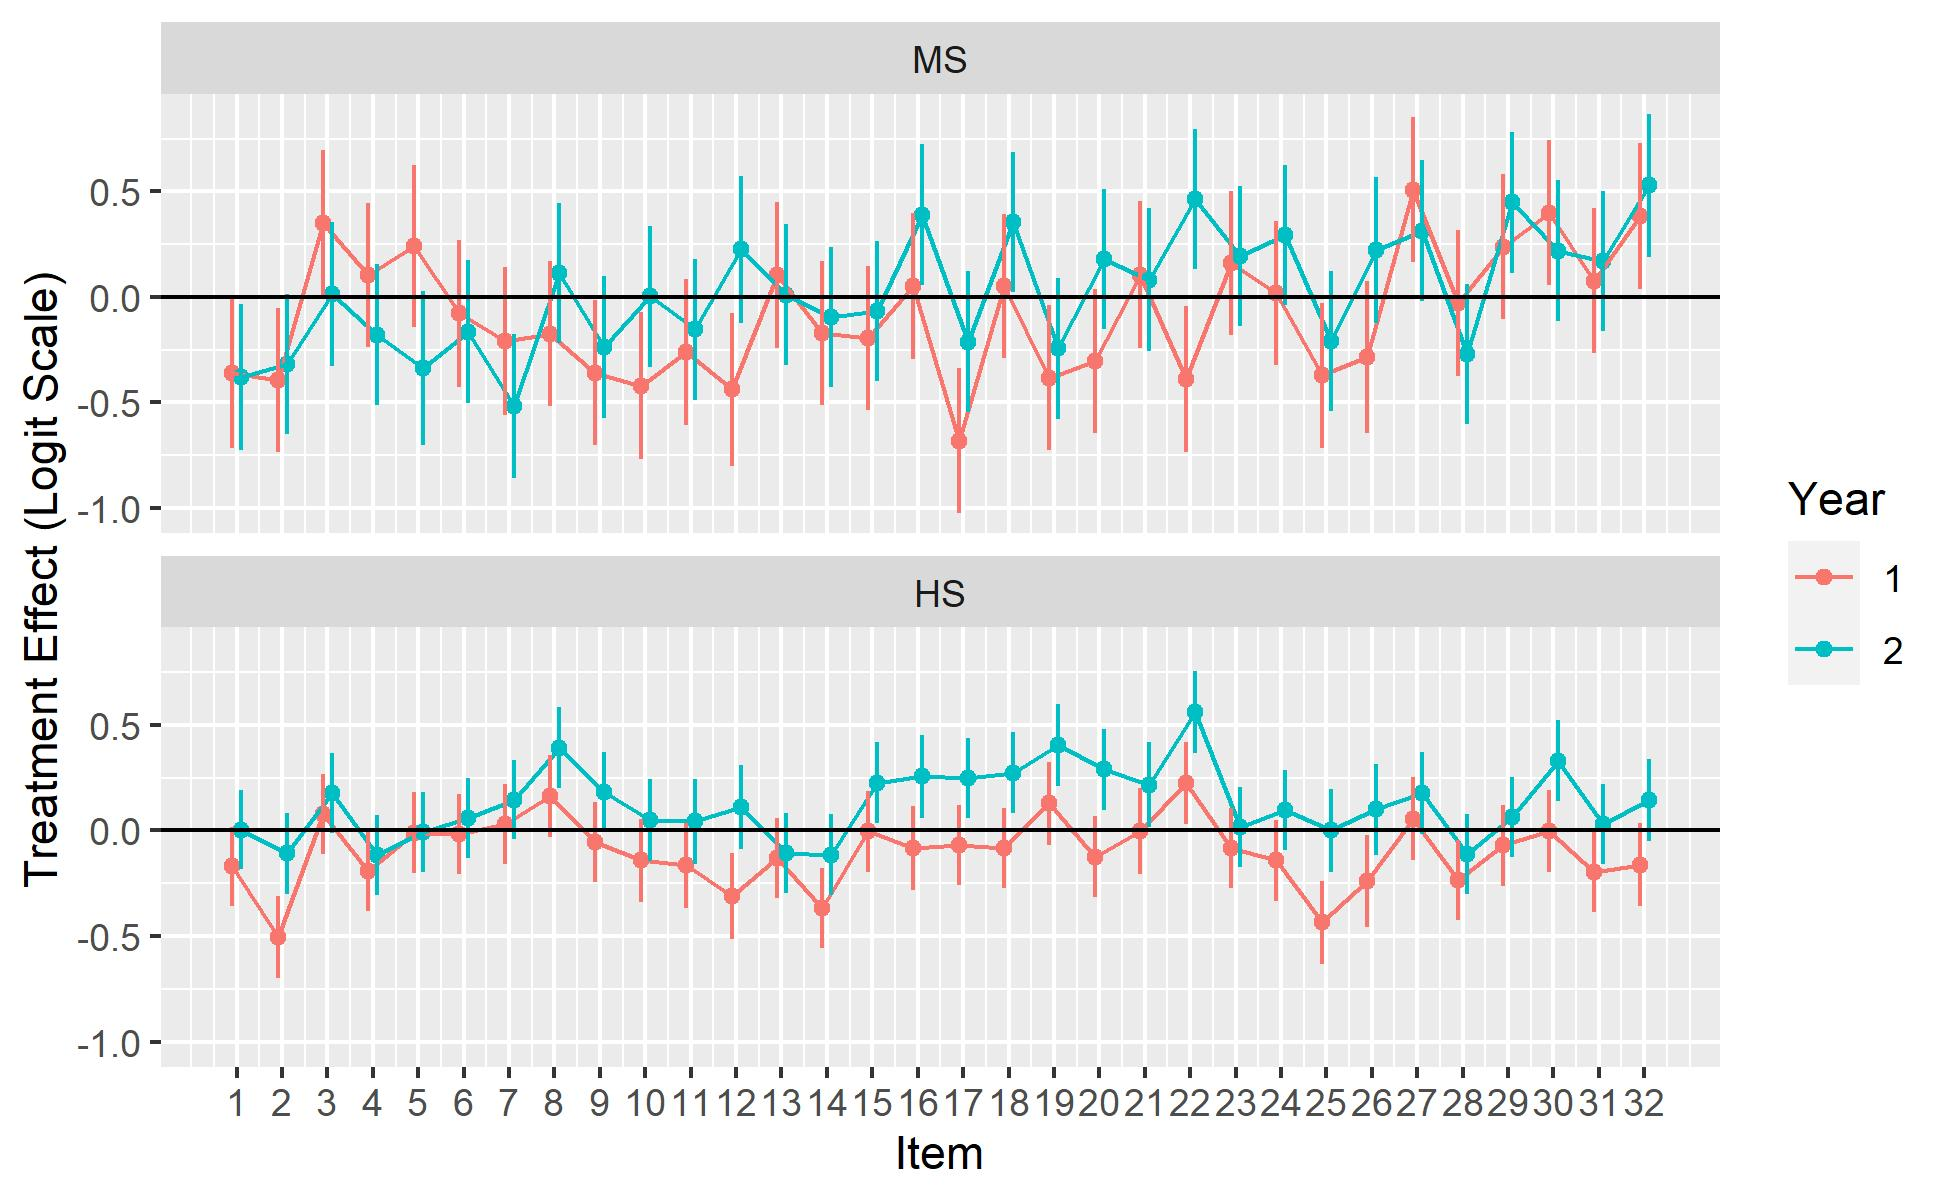
\includegraphics{../ctEffects.jpg}
\end{figure*}


\section{Exploring Hypotheses about \emph{Why} Effects Differed}

\subsection{Citations}
Citations to articles \cite{bowman:reasoning, clark:pct, braams:babel, herlihy:methodology},
conference
proceedings \cite{clark:pct} or books \cite{salas:calculus, Lamport:LaTeX} listed
in the Bibliography section of your
article will occur throughout the text of your article.
You should use BibTeX to automatically produce this bibliography;
you simply need to insert one of several citation commands with
a key of the item cited in the proper location in
the \texttt{.tex} file \cite{Lamport:LaTeX}.
The key is a short reference you invent to uniquely
identify each work; in this sample document, the key is
the first author's surname and a
word from the title.  This identifying key is included
with each item in the \texttt{.bib} file for your article.

The details of the construction of the \texttt{.bib} file
are beyond the scope of this sample document, but more
information can be found in the \textit{Author's Guide},
and exhaustive details in the \textit{\LaTeX\ User's
Guide}\cite{Lamport:LaTeX}.

This article shows only the plainest form
of the citation command, using \texttt{{\char'134}cite}.
This is what is stipulated in the SIGS style specifications.
No other citation format is endorsed.



\section{Conclusions}

%ACKNOWLEDGMENTS are optional
\section{Acknowledgments}
This section is optional; it is a location for you
to acknowledge grants, funding, editing assistance and
what have you.  In the present case, for example, the
authors would like to thank Gerald Murray of ACM for
his help in codifying this \textit{Author's Guide}
and the \textbf{.cls} and \textbf{.tex} files that it describes.

%
% The following two commands are all you need in the
% initial runs of your .tex file to
% produce the bibliography for the citations in your paper.
\bibliographystyle{abbrv}
\bibliography{sigproc}  % sigproc.bib is the name of the Bibliography in this case

\end{document}
